{ %section1_2
	\subsection{Термины и определения}
	\par\textbf{Параллельные вычисления} – 
способ организации вычислений, при котором программа представляет из себя набор взаимодействующих модулей, работающих одновременно. Как правило понятие параллелизма может включать:
		\begin{enumerate}
			\item\textbf{Параллелизм уровня инструкций} - одно ядро процессора может выполнять несколько инструкций одновременно. Например, такая технология реализована в процессорах Pentium 4 компании Intel.
			\item\textbf{Гипертрединг} - одно ядро процессора спроектировано так, что может выполнять работу сразу двух тредов. Реализована в процессорах серии Intel Core i7. При выполнении лабораторных работ важно отключать этот пункт в BIOS (если процессор совместим с данной технологией), так как он существенно влияет на показатели параллельного ускорения и эффективности.
			\item\textbf{Многоядерное программирование} -  способ решения вычислительных задач с одновременным выполнением частей программы на разных физических вычислительных ядрах. Все вычислительные ядра имеют общие банки памяти, так как находятся на одной вычислительной машине. Включает себя случай многоядерной архитектуры процессора и многопроцессорной архитектуры системы, в которой находится несколько процессоров, так как в обоих случаях программа выполняется на нескольких ядрах одного или множества процессоров, но на одной физической ЭВМ.
			\item\textbf{Распределенные вычисления} - способ решения трудоёмких вычислительных задач с использованием нескольких компьютеров, чаще всего объединённых в параллельную вычислительную систему. Разные части программы могут выполняться на разных компьютерах.
		\end{enumerate}
	Обычно последние два понятия физически реализуются с помощью архитектур \textit{SMP} и \textit{MMP}, подробнее о которых можно прочитать в следующем разделе.
	\parВажно различать понятия ''параллельные вычисления'' и ''параллельные технологии''. Разберем следующие понятия, которые, хотя и являются параллельными технологиями (на уровне ядра или межъядерного взаимодействия), однако не являются параллельными вычислениями, но часто \textbf{по ошибке} причисляются к ним:
		\begin{itemize}
			\item\textit{Конвейерная обработка данных (суперскалярность)} представляет собой одновременную обработку процессором нескольких инструкций, при котором в один момент времени для каждой из инструкций выполняется различный этап выполнения. Например, если какой-либо процессор может одновременно получать, раскодировать, и выполнить инструкцию, то он во время получения первой инструкции может раскодировать вторую и выполнять третью (рисунок~\ref{pipelineExample:image}). Этот способ организации вычислений не является параллельными вычислениями, потому что инструкции все равно выполняются последовательно, а так же задействовано только одно ядро.
				\begin{figure}[H]
					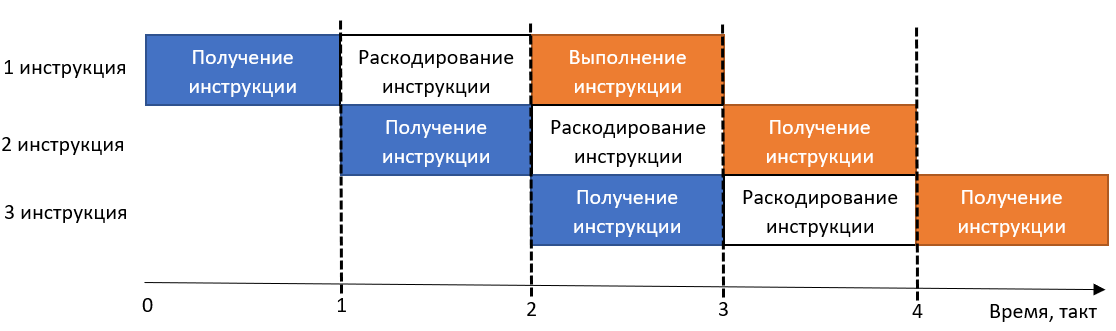
\includegraphics[width=1\linewidth]{pipelineExample}
					\caption{\textit{Конвейерная обработка инструкций}}
					\label{pipelineExample:image}
				\end{figure}
			\item\textit{SIMD-расширения (MMX, SSE)} обеспечивают параллелизм на уровне данных. Например, процессор может одновременно умножать 4 числа вместо одного с помощью SSE инструкции. Однако поток команд все равно остается одиночным, т.е. выполняется одна инструкция программы за промежуток времени, что не является случаем параллельных вычислений.
			\item\textit{Вытесняющая многозадачность} организуется операционной системой. Несколько процессов стоят в очереди выполнения и ОС сама решает как распорядиться процессорным временем между ними. Если у первого потока задан больший приоритет чем у второго, то ОС будет выделять больше времени на выполнение первого потока, одна в один момент времени будет выполняться только один поток, следовательно, вытесняющая многозадачность тоже не входит в понятие параллельных вычислений.
		\end{itemize}
	\parДля организации параллельных вычислений используются различные технологии распараллеливания:
		\begin{itemize}
			\item\textbf{Process (процесс)} - наиболее тяжеловесный механизм, применяемый для распараллеливания. Каждый процесс имеет свое независимое адресное пространство, поэтому синхронизация данных между процессами долгая и сложная. Может включать в себя несколько потоков исполнения.
			\item\textbf{Thread (поток исполнения, нить, тред, поток)} выполняется независимо от других потоков, но имеет общее адресное пространство с другими потоками в рамках одного процесса. На этом уровне используется механизмы синхронизации данных (будут рассмотрены далее).
			\item\textbf{Fiber (волокно)} - легковесный поток выполнения. Также как и треды, fiber'ы имеют общее адресное пространство, однако используют совместную многозадачность вместо вытесняющей. ОС не переключает контекст из одного треда в другой, вместо этого главный поток сам выделяет время для работы дочернего fiber, либо блокируется логически (то есть жизненным циклом fiber'a управляет программист). Также все fiber'ы работают на одном ядре, в отличии от тредов, которые могут работать на разных ядрах.
		\end{itemize}
	\parДля лучшего понимания тредов схематично рассмотрим его жизненный цикл (lifecycle). На рисунке~\ref{threadLifecycle:image} видно, что поток может находится в трех состояниях - готовность, ожидание и выполнение. После создания потока он пребывает в состоянии готовности. Затем ОС принимает решение о смене его состояния (вытесняющая многозадачность). Для fiber жизненный цикл такой же, но переходами между ними управляет программист или механизмы синхронизации.
	\parРазные стандарты языков программирования могут добавлять в жизненный цикл потоков новые состояния, например, блокировка потока, прерывание работы потока и остальные, однако общая схема работы остается той же.
		\begin{figure}[H]
			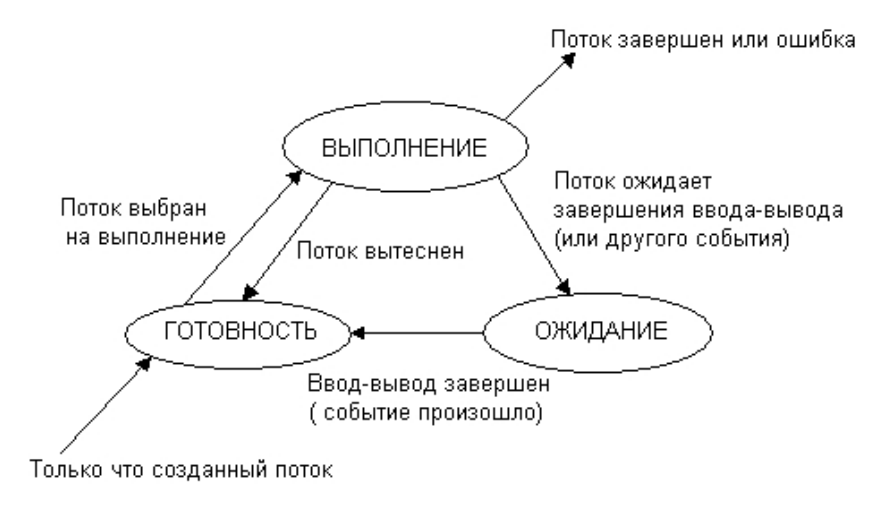
\includegraphics[width=0.9\linewidth]{threadLifecycle}
			\caption{\textit{Жизненный цикл потока}}
			\label{threadLifecycle:image}
		\end{figure}
	\parВ среде программистов существуют понятия \textbf{потокобезопасной (thread-safe)} и \textbf{реэнтерабельной (reentrant)} функции, однако в разных сообществах они могут иметь различные значения. В таблице~\ref{threadSafeReentrant:table} написаны определения из разных источников.
	\begin{table}[H]
		\caption{Определения thread-safe и reentrant функций}
		\label{threadSafeReentrant:table}
		\begin{center}
			%\begin{tabular}{c}
				%\begin{figure}[H]
					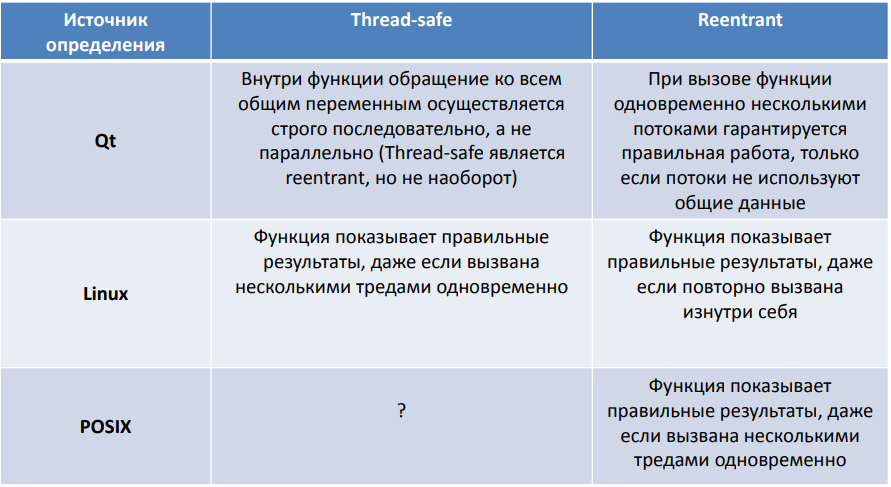
\includegraphics[width=1\linewidth]{parallelFunctionTypes}
				%\end{figure}
			%\end{tabular}
		\end{center}
	\end{table}
	\parРассмотрим примеры функций, подходящие под определение сообщества Linux.
	\begin{figure}[H]
		\lstinputlisting{swapExample1.cpp}
	\end{figure}
	\parДанная функция не является не потокобезопасной, не реентерабельной, потому что все потоки вызывающие ее будут использовать общую переменную t. Если вызвать функцию внутри ее самой, то перезапишется значение t и родительская функция отработает неправильно. Попробуем исправить эти ошибки, объявив переменную t типа \textunderscore \textunderscore threadint.
	\begin{figure}[H]
		\lstinputlisting{swapExample2.cpp}
	\end{figure}
	\parТеперь компилятор создаст копию переменной для каждого потока t и функция станет потокобезопасной, однако она все еще не реентерабельна по той же причине. Будем сохранять значение глобальной переменной t в начале функции и восстанавливать ее в конце.
	\begin{figure}[H]
		\lstinputlisting{swapExample3.cpp}
	\end{figure}
	\parНовая функция реентерабельна, но снова потоконебезопасна. Наконец, приведем пример стандартной и правильной реализации swap(), которая потокобезопасна и реентерабельна:
	\begin{figure}[H]
		\lstinputlisting{swapExample4.cpp}
	\end{figure}
}